\documentclass{article}

\usepackage[T1,T2A]{fontenc}
\usepackage[utf8]{inputenc}
\usepackage[english,russian]{babel}
\usepackage[14pt]{extsizes}

\usepackage[left=25mm,right=15mm,top=20mm,bottom=20mm,footskip=15mm,includefoot]{geometry}

\usepackage{graphicx}
\graphicspath{ {./pictures/} }

\usepackage{listings}

\begin{document}
    \pagenumbering{arabic}
    \tableofcontents{}
    \newpage

    \section{Введение}
    В настоящее время на одном диске в среднем записывается несколько десятков 
    тысяч файлов. Как разобраться во всем этом многообразии с тем, чтобы точно 
    адресоваться к файлу? Назначение файловой системы - эффективное решение 
    указанной задачи.

    Развитие файловых систем персональных компьютеров определялось двумя 
    факторами - появлением новых стандартов на носители информации и ростом 
    требований к характеристикам файловой системы со стороны прикладных 
    программ (разграничение уровней доступа, поддержка длинных имен файлов в 
    формате \texttt{UNICODE}). Первоначально, для файловых систем первостепенное 
    значение имело увеличение скорости доступа к данным и минимизация объема 
    хранимой служебной информации. Впоследствии с появлением более быстрых 
    жестких дисков и увеличением их объемов, на первый план вышло требование 
    надежности хранения информации, которое привело к необходимости избыточного 
    хранения данных.
    
    Эволюция файловой системы была напрямую связана с развитием технологий 
    реляционных баз данных. Файловая система использовала последние достижения, 
    разработанные для применения в СУБД: механизмы транзакций, защиты данных, 
    систему самовосстановления в результате сбоя.
    
    Развитие файловых систем привело к изменению самого понятия "файл" от 
    первоначального толкования как упорядоченная последовательность логических 
    записей, до понятия файла, как объекта, имеющего набор характеризующих его 
    атрибутов (включая имя файла, его псевдоним, время создания и собственно 
    данные).
    
    За свою 20 летнюю историю файловая система прошла путь от простой системы, 
    взявшей на себя функции управления файлами, до системы, представляющей 
    собой полноценную СУБД, обладающую встроенным механизмом протоколирования 
    и восстановления данных.
    
    В отличие от попыток ввести стандарт на протокол, описывающий правила 
    доступа к удаленным файловым системам, не стоит ожидать появления подобного 
    стандарта, описывающего файловые системы для жестких дисков. Это можно 
    объяснить тем, что файловая система жестких дисков все еще продолжает 
    оставаться одной из главных частей операционной системы, влияющей на ее 
    производительность. Поэтому каждый производитель операционных систем будет 
    стремиться использовать файловую систему, "родную" для его ОС.
    
    Дальнейшая эволюция файловых систем пойдет по пути совершенствования 
    механизмов хранения данных, оптимизации хранения мультимедийных данных, 
    использования новых технологий, применяемых в базах данных (возможность 
    полнотекстового поиска, сортировка файлов по различным атрибутам).

    \newpage

    \section{Основные термины и концепции \newline операционных систем}
    \subsection{Пользователь и ядро.}
    Пользователь и ядро - два термина, которые часто используются в 
    операционных системах. Их определение довольно прямолинейно: ядро - это
    часть операционной системы, которая работает с более высокими привилегиями, 
    в то время как пользователь (пространство) обычно означает приложения, 
    работающие с низкими привилегиями.

    Однако эти термины сильно перегружены и могут иметь очень специфические 
    значения в некоторых контекстах.

    Пользовательский режим и режим ядра - это термины, которые могут относиться 
    конкретно к режиму выполнения процессора. од, работающий в режиме ядра, 
    может полностью управлять процессором, в то время как код, работающий в 
    пользовательском режиме, имеет определенные ограничения. Например, 
    прерывания локального процессора можно отключить или включить 
    только во время работы в режиме ядра.

    Если такая операция выполняется во время работы в пользовательском режиме, 
    будет сгенерировано исключение, и ядро возьмет на себя его обработку.

    Пространство пользователя и пространство ядра могут относиться конкретно к 
    защите памяти или к виртуальным адресным пространствам, связанным либо с 
    ядром, либо с пользовательскими приложениями.

    Значительно упрощая, пространство ядра - это область памяти, которая 
    зарезервирована для ядра, а пространство пользователя - это область памяти, 
    зарезервированная для определенного пользовательского процесса. Доступ к 
    пространству ядра защищен, поэтому пользовательские приложения не могут 
    получить к нему прямой доступ, в то время как к пространству пользователя 
    можно получить прямой доступ из кода, запущенного в режиме ядра.

    \subsection{Стандартная архитектура операционной системы}
    В типичной архитектуре операционной системы ядро операционной системы 
    отвечает за доступ и совместное использование оборудования безопасным и 
    справедливым образом с несколькими приложениями.
     
    \newpage
    \begin{figure}[h]
        \center{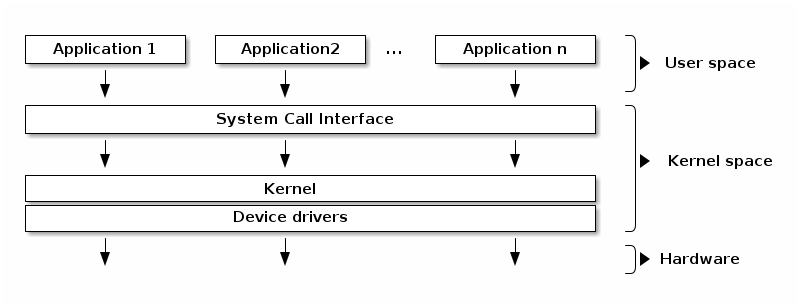
\includegraphics[width=\textwidth]{typical_os_arch.png}}
        \caption{Стандартная архитектура операционной системы}
    \end{figure} 

    Ядро предлагает набор API-интерфейсов, которые выдают приложения, которые 
    обычно называются «системными вызовами». Эти\\API-интерфейсы отличаются от 
    API-интерфейсов обычных библиотек, поскольку они являются границей, на 
    которой режим выполнения переключается из пользовательского режима в режим 
    ядра. 
    
    Чтобы обеспечить совместимость приложений, системные вызовы меняются 
    редко. Linux особенно это обеспечивает (в отличие от API ядра, которые могут
    изменяться по мере необходимости).

    Сам код ядра можно логически разделить на код ядра и код драйверов 
    устройств. Код драйверов устройств отвечает за доступ к определенным 
    устройствам, в то время как код ядра является общим. Ядро ядра можно 
    разделить на несколько логических подсистем (например, доступ к файлам, 
    работа в сети, управление процессами и т.д.).

    \section{Обзор ядра Linux}
    \subsection{Модель разработки Linux}
    Ядро Linux - это один из крупнейших проектов с открытым исходным кодом в 
    мире, в котором тысячи разработчиков вносят свой код, и миллионы строк кода 
    изменяются для каждого выпуска.

    Он распространяется под лицензией GPLv2, которая, проще говоря, требует, 
    чтобы любая модификация ядра, сделанная в программном обеспечении, 
    поставляемом заказчику, была доступна им (клиентам), хотя на практике 
    большинство компаний делают исходный код общедоступным.

    Есть много компаний (часто конкурирующих), которые вносят код в ядро Linux, 
    а также люди из академических кругов и независимые разработчики.

    Текущая модель разработки основана на выпуске релизов через фиксированные 
    промежутки времени (обычно 3-4 месяца). Новые функции объединяются в ядро в 
    течение одной или двух недель окна слияния. После окна слияния 
    выпуск-кандидат создается еженедельно (rc1, rc2 и т.д.).

    \subsection{Архитектура ядра Linux}

    \subsubsection{arch}
    \begin{itemize}
        \item Код для конкретной архитектуры
        \item Может быть дополнительно разделен на машинный код
        \item Взаимодействие с загрузчиком и инициализация, зависящая от
        архитектуры
        \item Доступ к различным аппаратным битам, например, контроллер
        прерываний, контроллеры SIMP, контроллеры шины, настройки исключений
        и прерываний, обработка виртуальной памяти
        \item Функции, оптимизированные для архитектуры (например memcpy)
    \end{itemize}

    Эта часть ядра Linux содержит архитектурно-зависимый код для определенных
    архитектур (например, arm).

    Первоначально Linux был разработан для 32-битных компьютеров на базе x86
    (386 или выше). В наши дни он также работает (по крайней мере) на Compaq
    Alpha AXP, Sun SPARC и UltraSparc, Motorola 68000, PowerPC, PowerPC64,
    ARM, Hitachi SuperH и др.

    \texttt{arch} реализует доступ к различным аппаратным битам, которые
    зависят от архитектуры или конкретной машины, например, контроллер
    прерываний, контроллеры SMP, контроллеры шины, настройки исключений и
    прерываний, обработка виртуальной памяти.

    \texttt{arch} также реализует функции, оптимизированные для архитектуры.

    \newpage
    \begin{figure}[h!]
        \center{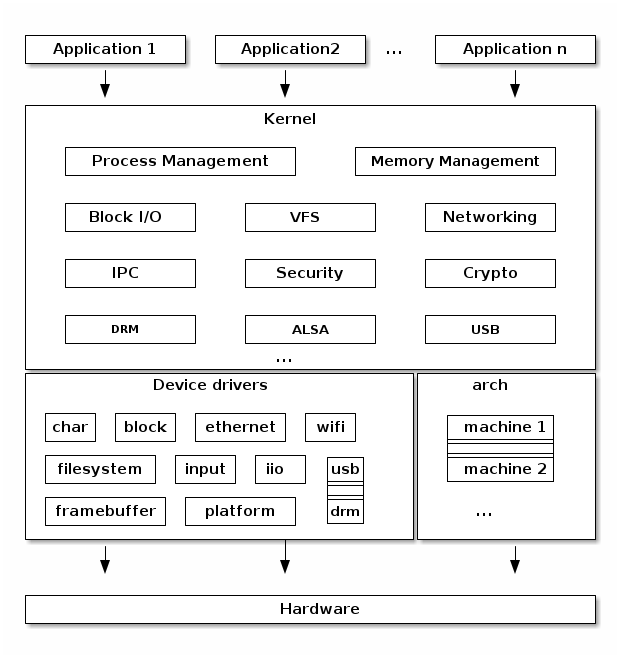
\includegraphics[width=\textwidth]{linux_arch.png}}
        \caption{Архитектура ядра линукс}
    \end{figure}

    \subsubsection{Device Drivers}
    Ядро Linux используют унифицированную модель устройства, цель которой -
    поддерживать внутренние структуры данных, отражающие состояние и
    структуру системы. Такая информация включает в себя, какие устройства
    присутствуют, каков их статус, к какой шине они подключены и т.д.
    Эта информация важна для реализации общесистемного управления питанием, а
    также обнаружения устройств и динамического удаления устройств.

    Каждая подсистема имеет свой собственный интерфейс драйвера, который
    адаптирован к устройствам, которые она представляет, чтобы упростить
    написание правильных драйверов и уменьшить дублирование кода.

    Linux поддерживает один из самых разнообразных наборов типов драйверов
    устройств.
    Некоторые примеры: TTY, SCSI, Ethernet, USB и т.д.

    \subsubsection{Process management}
    Linux реализует стандартные API-интерфейсы управления процессами \texttt{Unix}, такие
    как \texttt{fork()}, \texttt{exec}, \texttt{wait}, а также стандартные
    потоки \texttt{POSIX}.

    Однако процессы и потоки Linux реализован особенно иначе, чем другие ядра.
    Нет никаких внутренних структур, реализующих процессы или потоки, вместо
    этого есть \texttt{struct task\_struct}, которая описывает абстрактную
    единицу планирования, называемую задачей.

    Задача имеет указатели на ресурсы, такие как адресное пространство,
    дескрипторы файлов, идентификаторы \texttt{IPC} и т.д.
    Указатели ресурсов для задач, которые являются частью одного и того же
    процесса, указывают на одни и те же ресурсы, в то время как ресурсы задач
    разных процессов будут указывать на разные ресурсы.

    Эта особенность вместе с системными вызовами \texttt{clone()} и
    \texttt{unshare()} позволяет реализовать новые функции, такие как 
    пространство имен.

    Пространство имен используются вместе с контрольными группами (\texttt{cgroup})
    для реализации виртуализации операционной системы в Linux.

    \texttt{cgroup} - это механизм для иерархической организации процессов и
    распределения системных ресурсов по иерархии контролируемым и настраиваемым
    образом.

    \subsubsection{Memory management}
    Управление памятью Linux - это сложная подсистема, которая занимается:

    \begin{itemize}
        \item Управлением физической памятью: выделение и освобождение памяти;
        \item Управлением виртуальной памятью: подкачка, подкачка по запросу,
        копирование при записи
        \item Пользовательские сервисы: управление адресным пространством
        пользователя (например, \texttt{mmap()}, \texttt{brk()}, разделяемая 
        память)
        \item Сервисы ядра: распределители \texttt{SL*B}, \texttt{vmalloc}
    \end{itemize}

    \subsubsection{Block I/O management}
    Подсистема \texttt{Block I/O} Linux занимается чтением и записью данных с
    или на блочные устройства: создание запросов \texttt{Block I/O},
    преобразование запросов \texttt{Block I/O} (например, для программного
    \texttt{RAID} или \texttt{LVM}), объединение и сортировка запросов и их
    планирование через различные планировщики ввода-вывода для драйверов блочных
    устройств.

    \section{Управление файловыми системами в Linux}
    \subsection{Абстракции файловой системы}

    Файловая система - это способ организации файлов и каталогов на
    устройствах хранения, таких как жесткие диски, твердотелые накопители или
    флэш-память. Существует много типов файловых систем (например, \texttt{FAT},
    \texttt{ext4}, \texttt{btrfs}, \texttt{ntfs}), и в одной работающей системе
    мы можем использовать несколько экземпляров одного и того же типа файловой
    системы.

    Хотя файловые системы используют разные структуры данных для организации
    файлов, каталогов, пользовательских данных и метаданных (внутренних) на
    устройствах хранения, существует несколько общих абстракций, которые
    используются почти во всех файловых системах:

    \begin{itemize}
        \item \texttt{superblock}
        \item \texttt{file}
        \item \texttt{inode}
        \item \texttt{dentry}
    \end{itemize}

    Некоторые из этих абстракций присутствуют как на диске, так и в памяти, а
    некоторые - только в памяти.

    \texttt{superblock} содержит информацию об экземпляре файловой системы,
    такую как размер блока, корневой индексный дескриптор, размер файловой
    системы. Он присутствует как в хранилище, так и в памяти (для целей
    кеширования).

    \texttt{file} содержит информацию об открытом файле, такую как текущий
    указатель файла. \texttt{file} существует только в памяти.

    \texttt{inode} идентифицирует файл на диске. Он существует как в хранилище,
    так и в памяти (для кеширования). \texttt{inode} идентифицирует файл
    уникальным образом и имеет различные свойства, такие как размер файла,
    права доступа, тип файла и т.д.

    \texttt{dentry} связывает имя с индексным узлом. Он существует как в
    хранилище, так и в памяти (для кеширования).

    На рисунке \ref{fs} показана взаимосвязь между различными абстракциями файловой системы,
    используемыми в памяти.

    \begin{figure}[h!]
        \center{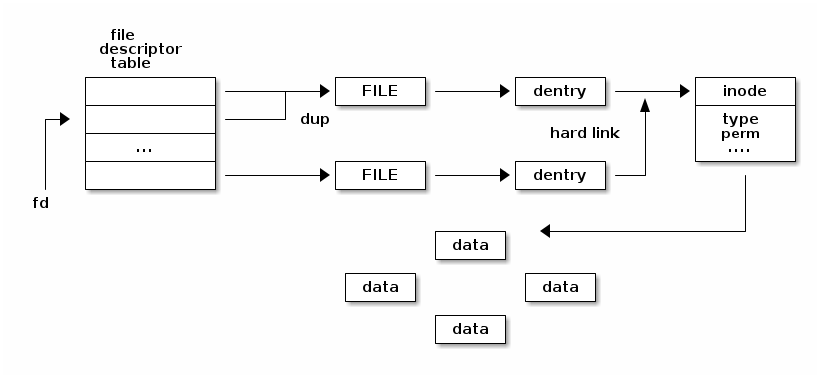
\includegraphics[width=\textwidth]{rel_fs.png}}
        \caption{Связь между различными абстракциями файловой системы}
        \label{fs}
    \end{figure}

    \subsection{Операции в файловых системах}
    На рисунке \ref{fs_dr} показана схема того, как драйверы файловой системы
    взаимодействуют с отсальной частью "стека" файловой системы. Для поддержки
    нескольких типов и экземпляров файловых систем, Linux реализует большую
    и сложную подсистему, которая занимается управлением файловой системой.
    Это называется виртуальной файловой системой и сокращенно \texttt{VFS}.

    \begin{figure}[h!]
        \center{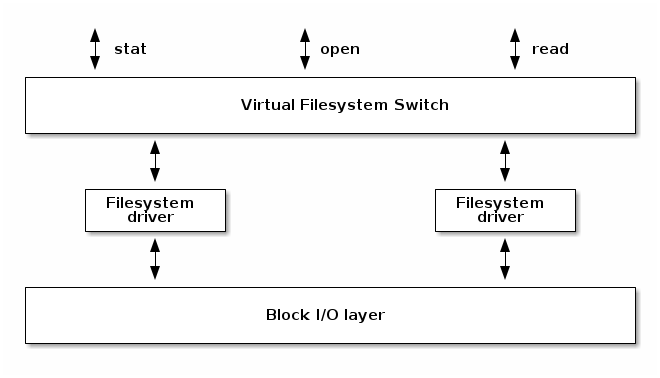
\includegraphics[width=\textwidth]{fs_dr.png}}
        \caption{Взаимодействие файловой системы с драйверами}
        \label{fs_dr}
    \end{figure}

    \texttt{VFS} преобразует сложные системные вызовы, связанные с управлением
    файлами, в более простые операции, которые реализуются драйверами устройств.
    Вот некоторые из операций, которые должна реализовывать файловая система:

    \begin{itemize}
        \item \texttt{mount}
        \item Открытие файла
        \item Запрос атрибутов файла
        \item Чтение данных из файла
        \item Запись файла в \texttt{file}
        \item Создание файла
        \item Удаление файла
    \end{itemize}

    \section{Разработка собственной файловой системы \newline $\texttt{treefs}$ для ядра Linux}
    \subsection{Регистрация файловой системы}
    Чтобы иметь возможность динамически загружать/выгружать модуль файловой
    системы, требуется \texttt{API} регистрации/отмены регистрации файловой
    системы. Структура, описывающая конкретную файловую систему, имеет вид
    \texttt{struct file\_system\_type}:

    \begin{lstlisting}
        #include <linux/fs.h>

        struct file_system_type {
            const char *name;
            int fs_flags;
            struct dentry *(*mount) (
                struct file_system_type *, int,
                const char *, void *,
            );
            void (*kill_sb) (struct super_block *);
            struct module *owner;
            struct file_system_type * next;
            struct hlist_head fs_supers;
            struct lock_class_key s_lock_key;
            struct lock_class_key s_umount_key;
            //...
        };
    \end{lstlisting}

    \begin{itemize}
        \item \texttt{name} - это строка, представляющая имя, которое будет
        идентифицировать файловую систему 
        (аргумент, переданный в \texttt{mount -t}).
        \item Владелец - \texttt{THIS\_MODULE} для файловых систем,
        реализованных в модулях, и \texttt{NULL}, если они записаны 
        непосредственно в ядро.
        \item Функция \texttt{mount} считывает \texttt{superblock} с диска
        памяти при загрузке файловой системы. Функция уникальна для каждой
        файловой системы.
        \item Функция \texttt{kill\_sb} освобождает \texttt{superblock} из
        памяти.
        \item \texttt{fs\_flags} указывает флаги, с которыми должна быть
        смонтирована файловая система. Примером такого флага является
        \texttt{FS\_REQUIRES\_DEV}, который указывает \texttt{VFS}, что
        файловой системе нужен диск.
        \item \texttt{fs\_super} - это список, содержащий все \texttt{superblock}, \newline
        связанные с этой файловой системой. Поскольку одну и ту же файловую
        систему можно монтировать несколько раз, для каждого монтирования
        будет отдельный \texttt{superblock}.
    \end{itemize}

    Регистрация файловой системы в ядре обычно выполняется в функции
    инициализации модуля. Для регистрации разработчику необходимо будет:

    \begin{itemize}
        \item Инициализировать структуру типа \texttt{struct file\_system\_type} \newline
        с именем, флагами, функцией, которая реализует операцию чтения суперблока
        и ссылкой на структуру, которая идентифицирует текущий модуль
        \item Вызвать функцию \texttt{register\_filesystem()}
    \end{itemize}

    При выгрузке модуля вы должны отменить регистрацию файловой системы, вызвав
    функцию \texttt{unregister\_filesystem()}.

    \subsection{\texttt{inode}}

    \texttt{inode} хранит информацию о файле: обычный файл, каталог, специальный
    файл (\texttt{pipe}, \texttt{fifo}), блочное устройство, символьное 
    устройство, ссылка или все, что можно абстрагировать как файл.

    \texttt{inode} хранит такую информацию как:

    \begin{itemize}
        \item тип файла
        \item размер файла
        \item права доступа
        \item доступ или изменение времени
        \item расположение данных на диске
    \end{itemize}

    \subsection{\texttt{VFS} в Linux}
    Хотя основной целью первоначального внедрения \texttt{VFS} в ядра 
    \texttt{UNIX} была поддержка нескольких типов и экземпляров файловых
    систем, побочным эффектом было то, что это упростило разработку
    драйверов устройств файловой системы, посколько части команд теперь
    реализованы в \texttt{VFS}. Практически все кэширование и управление
    буфером осуществляется с помощью \texttt{VFS}, оставляя только
    эффективное управление хранением данных драйверу устройства файловой
    системы.

    Чтобы иметь дело с несколькими типами файловых систем, \texttt{VFS}
    представила ранее представленные общие абстракции файловых систем. Обратите
    внимание, что драйвер файловой системы также может использовать свои
    собсвтенные абстракции файловой системы в памяти, и что также может быть
    другая абстракция в хранилище. Таким образом, мы можем получить три немного
    разные абстракции файловой системы: одну для \texttt{VFS} - всегда в памяти
    и две для конкретной файловой системы - одну в памяти, используемую драйвером
    файловом системы, и одну в хранилище.

    \newpage

    \begin{figure}[h!]
        \center{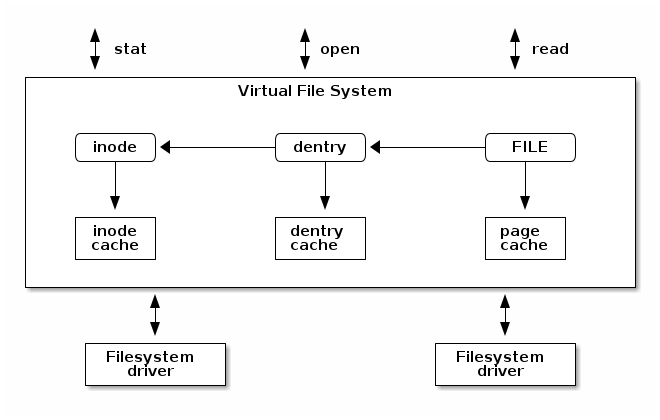
\includegraphics[width=\textwidth]{vfs.png}}
        \caption{Работа \texttt{VFS}}
    \end{figure}

    \subsection{\texttt{Superblock} в \texttt{VFS}}
    \texttt{superblock} существует как физический объект (объект на диске), так
    и как объект \texttt{VFS} (в \texttt{struct super\_block}).
    \texttt{superblock} содержит только метаинформацию и используется для
    записи и чтения метаданных с диска.
    \texttt{superblock} (и неявно \texttt{struct super\_block}) будет содержать
    информацию об используемом блочном устройстве, список индексных дескрипторов,
    указатель на индексный дескриптор корневого каталога файловой системы и
    указатель на операции \texttt{superblock}.

    \subsection{Алгоритм роста дерева}
    На начальной стадии был написан прототип роста дерева на языке
    \texttt{Python 3.9}. Этот инструмент очень хорошо подходит для быстрой
    реализации алгоритмов и их прототипирования.
    Задача состоит в реализации алгоритма роста дерева двух видов - береза и
    ель. Главное отличие в том, что "листьев" на березе меньше, чем на ели и
    через какое-то время и количество веток, они перестают расти.

    \begin{lstlisting}
# -*- coding: utf-8 -*-

import os
from uuid import uuid4


# Constants
CURR_PATH = os.getcwd()
YEARS = 10


def fib(num: int) -> int:
    """ Calculate fibonacci num """

    if num == -1: return 0
    if num == 0: return 0
    if num == 1: return 1
    return fib(num - 1) + fib(num - 2)


def touch(filename: str) -> None:
    """ Implements touch method """

    # Using append mode
    open(f'{CURR_PATH}/{filename}', 'a')


def mkdir(dirname: str) -> None:
    """ Implements mkdir method """
    os.mkdir(f'{CURR_PATH}/{dirname}')


class Leave:
    def __init__(
        self, 
        created_at: int, 
        branch: str,
    ) -> None:
        self.created_at = created_at
        self.path = \
          f'{branch}/leave_{self.created_at}_{uuid4().hex}'
        touch(self.path)


class Branch:
    def __init__(
        self, 
        created_at: int, 
        parent: str, 
        mode: str,
    ) -> None:
        # Save created year
        self.created_at: int = created_at

        self.path: str = \
          f'{parent}/branch_{self.created_at}_{uuid4().hex}'

        if mode == 'birch':
            self.num_of_leaves: int = 10
        else:
            self.num_of_leaves: int = 100

        self.leaves: list = []

        self.max_sub_branches_for_leaves: int = 5
        mkdir(self.path)

    @property
    def num_sub_branches(self) -> int:
        return len([d[0] for d in os.walk(self.path)]) - 1

    def is_old(
        self, 
        max_year: int, 
        current_year: int,
    ) -> bool:
        if current_year - self.created_at < max_year:
            return True
        return False

    def grow_leaves(self, year: int) -> None:
        if self.num_sub_branches <= \
          self.max_sub_branches_for_leaves:
            self.leaves: list = [
                Leave(year, self) for num \
                  in range(self.num_of_leaves)
            ]

    def __str__(self) -> str:
        return self.path


class Tree:
    def __init__(self, years: int, mode: str) -> None:
        self.years: int = years
        self.branches: list = []

        self.mode: str = mode
        mkdir(self.mode)
    
    def grow(self) -> None:
        if self.mode == 'birch':
            leaves_years_max: int = 3
        if self.mode == 'spruce':
            leaves_years_max: int = 1
        
        for year in range(self.years):
            self.branches.append(
                Branch(year, self.mode, self.mode)
            )
            for branch in self.branches:
                if not branch.is_old(
                    leaves_years_max, 
                    year,
                ):
                    for num in range(fib(year - 1)):
                        self.branches.append(
                            Branch(year, branch, self.mode),
                        )
                    branch.grow_leaves(year)

    
birch: Tree = Tree(YEARS, 'birch')
birch.grow()

spruce: Tree = Tree(YEARS, 'spruce')
spruce.grow()
    \end{lstlisting}

    После того, как был написан прототип на \texttt{Python 3.9} необходимо было
    реализовать этот алгоритм в коде файловой системы \texttt{treefs}.

    Класс \texttt{Tree} был реализован внутри структуры \texttt{treefs\_super\_block},
    а классы \texttt{Branch} и \texttt{Leave} внутри струкр \texttt{branch} и
    \texttt{leave} соответственно.

    \begin{lstlisting}
        struct leave {
            // Year that leave was created
            int created_at;
            // Leave name (path)
            char *name;
            unsigned long ino;
        };
        
        struct branch {
            // Year that branch was created
            int created_at;
            // Branch name (path)
            char *name;
        
            // Number of leaves on branch
            int num_of_leaves;
        
            int leaves_years_max;
        
            size_t current_num_of_leaves;
            size_t current_num_of_sub_branches;
        
            struct leave **leaves;
            struct branch **sub_branches;
        
            int max_sub_branches;
            int max_sub_branches_for_leaves;
            unsigned long ino;
        };
        
        enum treeType {
            birch,
            spruce,
        };
        
        
        struct treefs_super_block {
            struct timer_list treefs_timer;
            struct work_struct grow_struct;
            unsigned long next_ino;
        
            // Tree fields
            int years;
            int current_year;
            struct branch tree;
            enum treeType mode;
            size_t num_of_branches;
        }; 
    \end{lstlisting}

    Также был реализован метод \texttt{grow\_leaf} для роста "листьев".

    \begin{lstlisting}
    void grow_leaf(
        struct treefs_super_block *tsb, struct branch *b
    ) {
        struct leave *leaf;
        struct leave **new_leafs;
        struct leave **tmp_leafs;

        if (b->max_sub_branches ==
            b->max_sub_branches_for_leaves) {
            return;
        }

        // New leaf init for growing
        leaf = kzalloc(sizeof(*leaf), GFP_KERNEL);
        leaf->created_at = tsb->current_year;
        leaf->ino = tsb->next_ino++;

        new_leafs = kzalloc(
            sizeof(b->leaves) * 
            (b->current_num_of_leaves+1), 
            GFP_KERNEL
        );
        memcpy(
            new_leafs, 
            b->leaves, 
            sizeof(new_leafs[0])*b->current_num_of_leaves
        );
        new_leafs[b->num_of_leaves++] = leaf;
        tmp_leafs = b->leaves;
        b->leaves = new_leafs;
        kvfree(tmp_leafs);

    }
    \end{lstlisting}

    И рекурсивная функция \texttt{grow\_branch} для роста "веток".
    \begin{lstlisting}
    \end{lstlisting}

    \newpage
    \section{Заключение}
    В данной работе была рассмотрена архитектура ядра Linux, в частности
    внутреннее устройство и работа файловых систем, а также была разработана
    собсвтенная файловая система для ядра Linux, которая способна имплементировать
    два вида дерева - береза и ель.

    \newpage

    \begin{thebibliography}{99}
    \end{thebibliography}

    \newpage

    \section{Приложение}

\end{document}